% Options for packages loaded elsewhere
\PassOptionsToPackage{unicode}{hyperref}
\PassOptionsToPackage{hyphens}{url}
%
\documentclass[
  man,floatsintext]{apa6}
\usepackage{amsmath,amssymb}
\usepackage{iftex}
\ifPDFTeX
  \usepackage[T1]{fontenc}
  \usepackage[utf8]{inputenc}
  \usepackage{textcomp} % provide euro and other symbols
\else % if luatex or xetex
  \usepackage{unicode-math} % this also loads fontspec
  \defaultfontfeatures{Scale=MatchLowercase}
  \defaultfontfeatures[\rmfamily]{Ligatures=TeX,Scale=1}
\fi
\usepackage{lmodern}
\ifPDFTeX\else
  % xetex/luatex font selection
\fi
% Use upquote if available, for straight quotes in verbatim environments
\IfFileExists{upquote.sty}{\usepackage{upquote}}{}
\IfFileExists{microtype.sty}{% use microtype if available
  \usepackage[]{microtype}
  \UseMicrotypeSet[protrusion]{basicmath} % disable protrusion for tt fonts
}{}
\makeatletter
\@ifundefined{KOMAClassName}{% if non-KOMA class
  \IfFileExists{parskip.sty}{%
    \usepackage{parskip}
  }{% else
    \setlength{\parindent}{0pt}
    \setlength{\parskip}{6pt plus 2pt minus 1pt}}
}{% if KOMA class
  \KOMAoptions{parskip=half}}
\makeatother
\usepackage{xcolor}
\usepackage{longtable,booktabs,array}
\usepackage{calc} % for calculating minipage widths
% Correct order of tables after \paragraph or \subparagraph
\usepackage{etoolbox}
\makeatletter
\patchcmd\longtable{\par}{\if@noskipsec\mbox{}\fi\par}{}{}
\makeatother
% Allow footnotes in longtable head/foot
\IfFileExists{footnotehyper.sty}{\usepackage{footnotehyper}}{\usepackage{footnote}}
\makesavenoteenv{longtable}
\usepackage{graphicx}
\makeatletter
\def\maxwidth{\ifdim\Gin@nat@width>\linewidth\linewidth\else\Gin@nat@width\fi}
\def\maxheight{\ifdim\Gin@nat@height>\textheight\textheight\else\Gin@nat@height\fi}
\makeatother
% Scale images if necessary, so that they will not overflow the page
% margins by default, and it is still possible to overwrite the defaults
% using explicit options in \includegraphics[width, height, ...]{}
\setkeys{Gin}{width=\maxwidth,height=\maxheight,keepaspectratio}
% Set default figure placement to htbp
\makeatletter
\def\fps@figure{htbp}
\makeatother
\setlength{\emergencystretch}{3em} % prevent overfull lines
\providecommand{\tightlist}{%
  \setlength{\itemsep}{0pt}\setlength{\parskip}{0pt}}
\setcounter{secnumdepth}{-\maxdimen} % remove section numbering
% Make \paragraph and \subparagraph free-standing
\ifx\paragraph\undefined\else
  \let\oldparagraph\paragraph
  \renewcommand{\paragraph}[1]{\oldparagraph{#1}\mbox{}}
\fi
\ifx\subparagraph\undefined\else
  \let\oldsubparagraph\subparagraph
  \renewcommand{\subparagraph}[1]{\oldsubparagraph{#1}\mbox{}}
\fi
\newlength{\cslhangindent}
\setlength{\cslhangindent}{1.5em}
\newlength{\csllabelwidth}
\setlength{\csllabelwidth}{3em}
\newlength{\cslentryspacingunit} % times entry-spacing
\setlength{\cslentryspacingunit}{\parskip}
\newenvironment{CSLReferences}[2] % #1 hanging-ident, #2 entry spacing
 {% don't indent paragraphs
  \setlength{\parindent}{0pt}
  % turn on hanging indent if param 1 is 1
  \ifodd #1
  \let\oldpar\par
  \def\par{\hangindent=\cslhangindent\oldpar}
  \fi
  % set entry spacing
  \setlength{\parskip}{#2\cslentryspacingunit}
 }%
 {}
\usepackage{calc}
\newcommand{\CSLBlock}[1]{#1\hfill\break}
\newcommand{\CSLLeftMargin}[1]{\parbox[t]{\csllabelwidth}{#1}}
\newcommand{\CSLRightInline}[1]{\parbox[t]{\linewidth - \csllabelwidth}{#1}\break}
\newcommand{\CSLIndent}[1]{\hspace{\cslhangindent}#1}
\ifLuaTeX
\usepackage[bidi=basic]{babel}
\else
\usepackage[bidi=default]{babel}
\fi
\babelprovide[main,import]{english}
% get rid of language-specific shorthands (see #6817):
\let\LanguageShortHands\languageshorthands
\def\languageshorthands#1{}
% Manuscript styling
\usepackage{upgreek}
\captionsetup{font=singlespacing,justification=justified}

% Table formatting
\usepackage{longtable}
\usepackage{lscape}
% \usepackage[counterclockwise]{rotating}   % Landscape page setup for large tables
\usepackage{multirow}		% Table styling
\usepackage{tabularx}		% Control Column width
\usepackage[flushleft]{threeparttable}	% Allows for three part tables with a specified notes section
\usepackage{threeparttablex}            % Lets threeparttable work with longtable

% Create new environments so endfloat can handle them
% \newenvironment{ltable}
%   {\begin{landscape}\centering\begin{threeparttable}}
%   {\end{threeparttable}\end{landscape}}
\newenvironment{lltable}{\begin{landscape}\centering\begin{ThreePartTable}}{\end{ThreePartTable}\end{landscape}}

% Enables adjusting longtable caption width to table width
% Solution found at http://golatex.de/longtable-mit-caption-so-breit-wie-die-tabelle-t15767.html
\makeatletter
\newcommand\LastLTentrywidth{1em}
\newlength\longtablewidth
\setlength{\longtablewidth}{1in}
\newcommand{\getlongtablewidth}{\begingroup \ifcsname LT@\roman{LT@tables}\endcsname \global\longtablewidth=0pt \renewcommand{\LT@entry}[2]{\global\advance\longtablewidth by ##2\relax\gdef\LastLTentrywidth{##2}}\@nameuse{LT@\roman{LT@tables}} \fi \endgroup}

% \setlength{\parindent}{0.5in}
% \setlength{\parskip}{0pt plus 0pt minus 0pt}

% Overwrite redefinition of paragraph and subparagraph by the default LaTeX template
% See https://github.com/crsh/papaja/issues/292
\makeatletter
\renewcommand{\paragraph}{\@startsection{paragraph}{4}{\parindent}%
  {0\baselineskip \@plus 0.2ex \@minus 0.2ex}%
  {-1em}%
  {\normalfont\normalsize\bfseries\itshape\typesectitle}}

\renewcommand{\subparagraph}[1]{\@startsection{subparagraph}{5}{1em}%
  {0\baselineskip \@plus 0.2ex \@minus 0.2ex}%
  {-\z@\relax}%
  {\normalfont\normalsize\itshape\hspace{\parindent}{#1}\textit{\addperi}}{\relax}}
\makeatother

% \usepackage{etoolbox}
\makeatletter
\patchcmd{\HyOrg@maketitle}
  {\section{\normalfont\normalsize\abstractname}}
  {\section*{\normalfont\normalsize\abstractname}}
  {}{\typeout{Failed to patch abstract.}}
\patchcmd{\HyOrg@maketitle}
  {\section{\protect\normalfont{\@title}}}
  {\section*{\protect\normalfont{\@title}}}
  {}{\typeout{Failed to patch title.}}
\makeatother

\usepackage{xpatch}
\makeatletter
\xapptocmd\appendix
  {\xapptocmd\section
    {\addcontentsline{toc}{section}{\appendixname\ifoneappendix\else~\theappendix\fi\\: #1}}
    {}{\InnerPatchFailed}%
  }
{}{\PatchFailed}
\keywords{anorexia nervosa, reinforcement learning, contextual learning, probabilistic reversal learning\newline\indent Word count: X}
\usepackage{lineno}

\linenumbers
\usepackage{csquotes}
\usepackage{amsmath, xcolor, hyperref, svg, url, array, tabularx, booktabs, caption, float, resizegather, verbatim,threeparttable, caption, soul, pdflscape, longtable,  setspace, adjustbox, threeparttable, booktabs, longtable, makecell, rotating, afterpage, tabularx}
\newcommand{\comm}[1]{\ignorespaces}
\raggedbottom
\ifLuaTeX
  \usepackage{selnolig}  % disable illegal ligatures
\fi
\IfFileExists{bookmark.sty}{\usepackage{bookmark}}{\usepackage{hyperref}}
\IfFileExists{xurl.sty}{\usepackage{xurl}}{} % add URL line breaks if available
\urlstyle{same}
\hypersetup{
  pdftitle={Impact of Contextual Learning on Reinforcement Learning Performance in Anorexia Nervosa},
  pdfauthor={Corrado Caudek1 \& Ernst-August Doelle1,2},
  pdflang={en-EN},
  pdfkeywords={anorexia nervosa, reinforcement learning, contextual learning, probabilistic reversal learning},
  hidelinks,
  pdfcreator={LaTeX via pandoc}}

\title{Impact of Contextual Learning on Reinforcement Learning Performance in Anorexia Nervosa}
\author{Corrado Caudek\textsuperscript{1} \& Ernst-August Doelle\textsuperscript{1,2}}
\date{}


\shorttitle{CONTEXTUAL LEARNING IN AN}

\authornote{

Add complete departmental affiliations for each author here. Each new line herein must be indented, like this line.

Enter author note here.

The authors made the following contributions. Corrado Caudek: Conceptualization, Writing - Original Draft Preparation, Writing - Review \& Editing; Ernst-August Doelle: Writing - Review \& Editing, Supervision.

Correspondence concerning this article should be addressed to Corrado Caudek, Postal address. E-mail: \href{mailto:my@email.com}{\nolinkurl{my@email.com}}

}

\affiliation{\vspace{0.5cm}\textsuperscript{1} Wilhelm-Wundt-University\\\textsuperscript{2} Konstanz Business School}

\abstract{%
\textbf{Objective:} This study compared individuals with Restrictive Anorexia Nervosa (R-AN; n = 40) to Healthy Controls (HCs; n = 45) and healthy controls at RIsk of eating disorders (RI; n = 36) in a Probabilistic Reversal Learning (PRL) task. The aim was to investigate whether R-AN individuals perform similarly to HCs and RIs in neutral contexts but show significant impairments in food-related contexts. \textbf{Method:} Participants completed a PRL task, making choices related to their disorder or unrelated to it. \textbf{Results:} R-AN individuals showed lower learning rates for disorder-related decisions, but their performance on neutral decisions was similar to the HC and RI groups. Additionally, only the R-AN patients exhibited reduced learning rates for food-related decisions compared to food-unrelated decisions. \textbf{Discussion:} These findings suggest that contextual cues, like food images, negatively impact Reinforcement Learning (RL) processes in individuals with R-AN. This raises questions about whether the impaired RL performance should be solely attributed to compromised learning mechanisms, especially when RL abilities appear intact in neutral contexts. The study's insights may have implications for developing interventions that target decision-making processes in individuals with R-AN.
}



\begin{document}
\maketitle

\hypertarget{introduction}{%
\section{Introduction}\label{introduction}}

Anorexia Nervosa (AN) is one of the most common eating disorders characterized by distorted body perception and pathological weight loss, particularly in its restricting type (R-AN) (American Psychiatric Association, 2022). Lifetime prevalence for AN has been reported at 1.4\% for women and 0.2\% for men (Galmiche, Déchelotte, Lambert, \& Tavolacci, 2019; Smink, Hoeken, \& Hoek, 2013), with a mortality rate that can be as high as 5-20\% (Qian et al., 2022). Treating AN is extremely challenging (Atwood \& Friedman, 2020; Linardon, Fairburn, Fitzsimmons-Craft, Wilfley, \& Brennan, 2017), highlighting the importance of gaining a deeper understanding of its underlying mechanisms (Chang, Delgadillo, \& Waller, 2021).

Executive functions have gained significant attention in the research on understanding the mechanisms underlying AN. Impairments in executive processes, such as cognitive inflexibility, decision-making difficulties, and inhibitory control problems, have been identified as potential risk and perpetuating factors in AN (Bartholdy, Dalton, O'Daly, Campbell, \& Schmidt, 2016; Guillaume et al., 2015; Wu et al., 2014). In particular, cognitive inflexibility in AN refers to difficulties adapting thoughts and actions to new information. This rigidity can lead to repetitive behaviors. On the other hand, reinforcement learning is the brain's way of optimizing decision-making based on action outcomes, where positive outcomes encourage repetition and negative outcomes discourage it. In AN, cognitive inflexibility can hinder updating of action-outcome associations, affecting adaptive behavior learning and leading to impaired reinforcement learning processes. This may contribute to difficulties recognizing the negative consequences of restrictive eating behaviors, perpetuating the disorder. While studies have explored reward processing abnormalities, our understanding of learning-related anomalies in AN remains limited (Schaefer \& Steinglass, 2021).

In relation to dysfunctions reward responsiveness among individuals with AN, research has revealed that the intense levels of dietary restriction and physical activity typically associated with AN can trigger the activation of reward pathways in the brain (Keating, 2010; Keating, Tilbrook, Rossell, Enticott, \& Fitzgerald, 2012; Selby \& Coniglio, 2020). Additionally, individuals with AN may exhibit diminished reward responses specifically towards food-related stimuli (Wierenga et al., 2014). In a broader sense, research has shown that AN is associated with reduced subjective reward sensitivity and decreased neural response to rewarding stimuli. Moreover, individuals with AN may experience disruptions in processing aversive stimuli, leading to heightened harm avoidance, reduced tolerance for uncertainty, increased anxiety, and heightened sensitivity to punishment (Fladung, Schulze, Schöll, Bauer, \& Groen, 2013; Jappe et al., 2011; Keating et al., 2012; O'Hara, Campbell, \& Schmidt, 2015). These factors collectively contribute to an altered response to negative feedback and a propensity to actively avoid aversive outcomes (Jonker, Glashouwer, \& Jong, 2022; Matton, Goossens, Braet, \& Vervaet, 2013). Neuroimaging studies have further supported these findings by revealing neural dysfunctions in individuals with AN regarding their response to loss and aversive taste stimuli (Bischoff-Grethe et al., 2013; Monteleone et al., 2017; Wagner et al., 2007).

Given the crucial importance of RL in acquiring knowledge from past experiences, extensive research has been conducted to examine potential deficits in RL among individuals diagnosed with AN (Bischoff-Grethe et al., 2013; Glashouwer, Bloot, Veenstra, Franken, \& Jong, 2014; Harrison, Genders, Davies, Treasure, \& Tchanturia, 2011; Jappe et al., 2011; Matton et al., 2013). However, the findings of these studies have been mixed. For example, Ritschel et al. (2017) found that individuals who had recovered from AN had impaired RL performance compared to healthy controls (HCs) on a Probabilistic Reversal Learning (PRL) task, particularly in response to negative feedback. In contrast, Bernardoni et al. (2018) found that AN patients had a higher learning rate from punishment than HCs. Similarly, Sarrar et al. (2016) found no differences in task performance between individuals with acute AN and HCs using the Probabilistic Object Reversal Task with neutral stimuli. Geisler et al. (2017) also found no group differences in a PRL task with neutral stimuli and monetary feedback.

To shed light on the potential reinforcement RL deficits in AN, researchers have incorporated food-related information into the PRL paradigm. For example, Zhang, Manson, Schiller, and Levy (2014) found that individuals with binge-eating disorder (BED) exhibited poorer performance when exposed to food-related feedback, indicating a vulnerability to food-related cues. However, attempts to replicate these findings in AN have yielded conflicting results. Hildebrandt et al. (2015) reported increased inflexibility in AN individuals using a PRL task with food-related feedback, while Hildebrandt et al. (2018) found no differences in PRL performance between AN patients and healthy controls (HCs) when employing the same paradigm.

Given the inconsistent findings in behavioral experiments regarding RL in AN, we propose that these discrepancies may be partly attribute to the predominant use of general stimuli instead of stimuli specifically relevant to the disorder (Schaefer \& Steinglass, 2021). Furthermore, when disorder-related information has been incorporated, it has typically been limited to the feedback provided after the participant's choice, with the stimuli presented during the decision-making process unrelated to the disorder. This approach primarily emphasizes the consequences of the choices, neglecting the contextual factors surrounding the decision-making process.

From a theoretical perspective, the methodological choices made in previous studies overlook the critical role of context in learning processes. Contextual learning (Heald, Lengyel, \& Wolpert, 2023) draws upon the notion, grounded in the human memory literature, that memory retrieval depends on the match between the conditions during learning and testing. When there is a mismatch, retrieval is impaired. Applying this concept to RL in AN (Rosas, Todd, \& Bouton, 2013), it can be hypothesized that contextual factors, such as individual characteristics, long-term goals, and situational influences, can contribute to impaired RL specifically in decision-making related to the disorder. This impairment can occur even when RL performance remains intact for decisions unrelated to the disorder (Haynos, Widge, Anderson, \& Redish, 2022). In other words, we propose that intermittent impaired RL performance in AN may arise from contextual factors that activate specific learning modes, rather than indicating a fundamental alteration in the underlying learning processes in the brain (for a discussion, see Bernardoni et al., 2021).

To examine the proposed hypothesis, we conducted a study using a modified version of the standard PRL task. Unlike previous studies that used general stimuli (Schaefer \& Steinglass, 2021), our task incorporated two distinct contexts. In one context, participants made choices between a stimulus related to the disorder (e.g., a caloric food) and a stimulus unrelated to the disorder (e.g., a lamp). In the other context, participants made choices between two stimuli unrelated to the disorder (i.e., flower vs.~objects).

Based on the responses to food stimuli often seen in individuals with AN, which typically exhibit reduced reward, increased aversion, and inhibition (Haynos, Lavender, Nelson, Crow, \& Peterson, 2020), we hypothesized that there would be a more conservative learning rate for disorder-related choices compared to disorder-unrelated choices within a PRL task. Additionally, we anticipated a lower learning rate for disorder-related choices in individuals with AN compared to HCs. Conversely, we expected no learning abnormalities in individuals with AN for choices unrelated to the disorder.

\hypertarget{methods}{%
\section{Methods}\label{methods}}

The study, which adhered to the Declaration of Helsinki, was approved by the University of Florence's Ethical Committee (Prot. n.~0178082). All eligible participants provided informed consent and willingly agreed to participate in the study.

\hypertarget{participants}{%
\subsection{Participants}\label{participants}}

The study included 40 individuals diagnosed with Restricting-Type Anorexia Nervosa (R-AN) according to the DSM-5 criteria and 45 healthy volunteers (Table 2). The participants with R-AN were recruited from three facilities in Italy: the Specchidacqua Institute in Montecatini (Pisa), the Villa dei Pini Institute in Firenze, and the Gruber Center, Outpatient Clinic in Bologna. The treatment approach consisted of Cognitive Behavioral Therapy and family-based treatment, with patients receiving treatment for 2 to 6 hours per day, 2 days per week. The treatment program included various components such as individual therapy, family therapy, group therapy, nutritional counseling, psychiatric care, and medical monitoring. The diagnosis of AN was made by specialized psychiatrists and psychologists through a semi-structured interview based on the DSM-5 criteria, at the start of treatment.

The study recruited additional 310 female adolescents or young adults through social media or university advertisements, and they completed the Eating Attitudes Test-26 (EAT-26) screening tool. Those scoring above 20 on the EAT-26 and not receiving current treatment for eating disorders were classified as ``at-risk'' {[}RI; Dotti and Lazzari (1998){]}, resulting in 36 individuals. From the remaining participants scoring below 20 on the EAT-26 and not receiving current treatment for eating disorders, 45 females were randomly selected and assigned to the healthy control (HC) group. Both the RI and HC groups had participants with a normal Body Mass Index (BMI). More details about eligibility criteria and sample characteristics can be found in the Supplementary Information (SI).

\hypertarget{procedure}{%
\subsection{Procedure}\label{procedure}}

In the initial session, participants underwent a clinical interview to determine their eligibility for the study. Those who met the criteria proceeded to anthropometric measurements and completed a battery of psychometric scales: the Eating Attitude Test (EAT-26; Garner (1991)), the Body Shape Questionnaire-14 {[}BSQ-14; Dowson and Henderson (2001){]}, the Social Interaction Anxiety Scale {[}SIAS; Mattick and Clarke (1998){]}, the Depression Anxiety Stress Scale-21 {[}DASS-21; Lovibond and Lovibond (1995){]}, the Rosenberg Self-Esteem Scale {[}RSES; Rosenberg (1965){]}, and the Multidimensional Perfectionism Scale {[}MPS-F; Frost, Marten, Lahart, and Rosenblate (1990){]}. In a subsequent session, participants completed the PRL task. Participants were told they would be playing a simple computer game with the objective of accumulating as many ``virtual euro'' as possible (see Figure 1).



\begin{figure}

{\centering 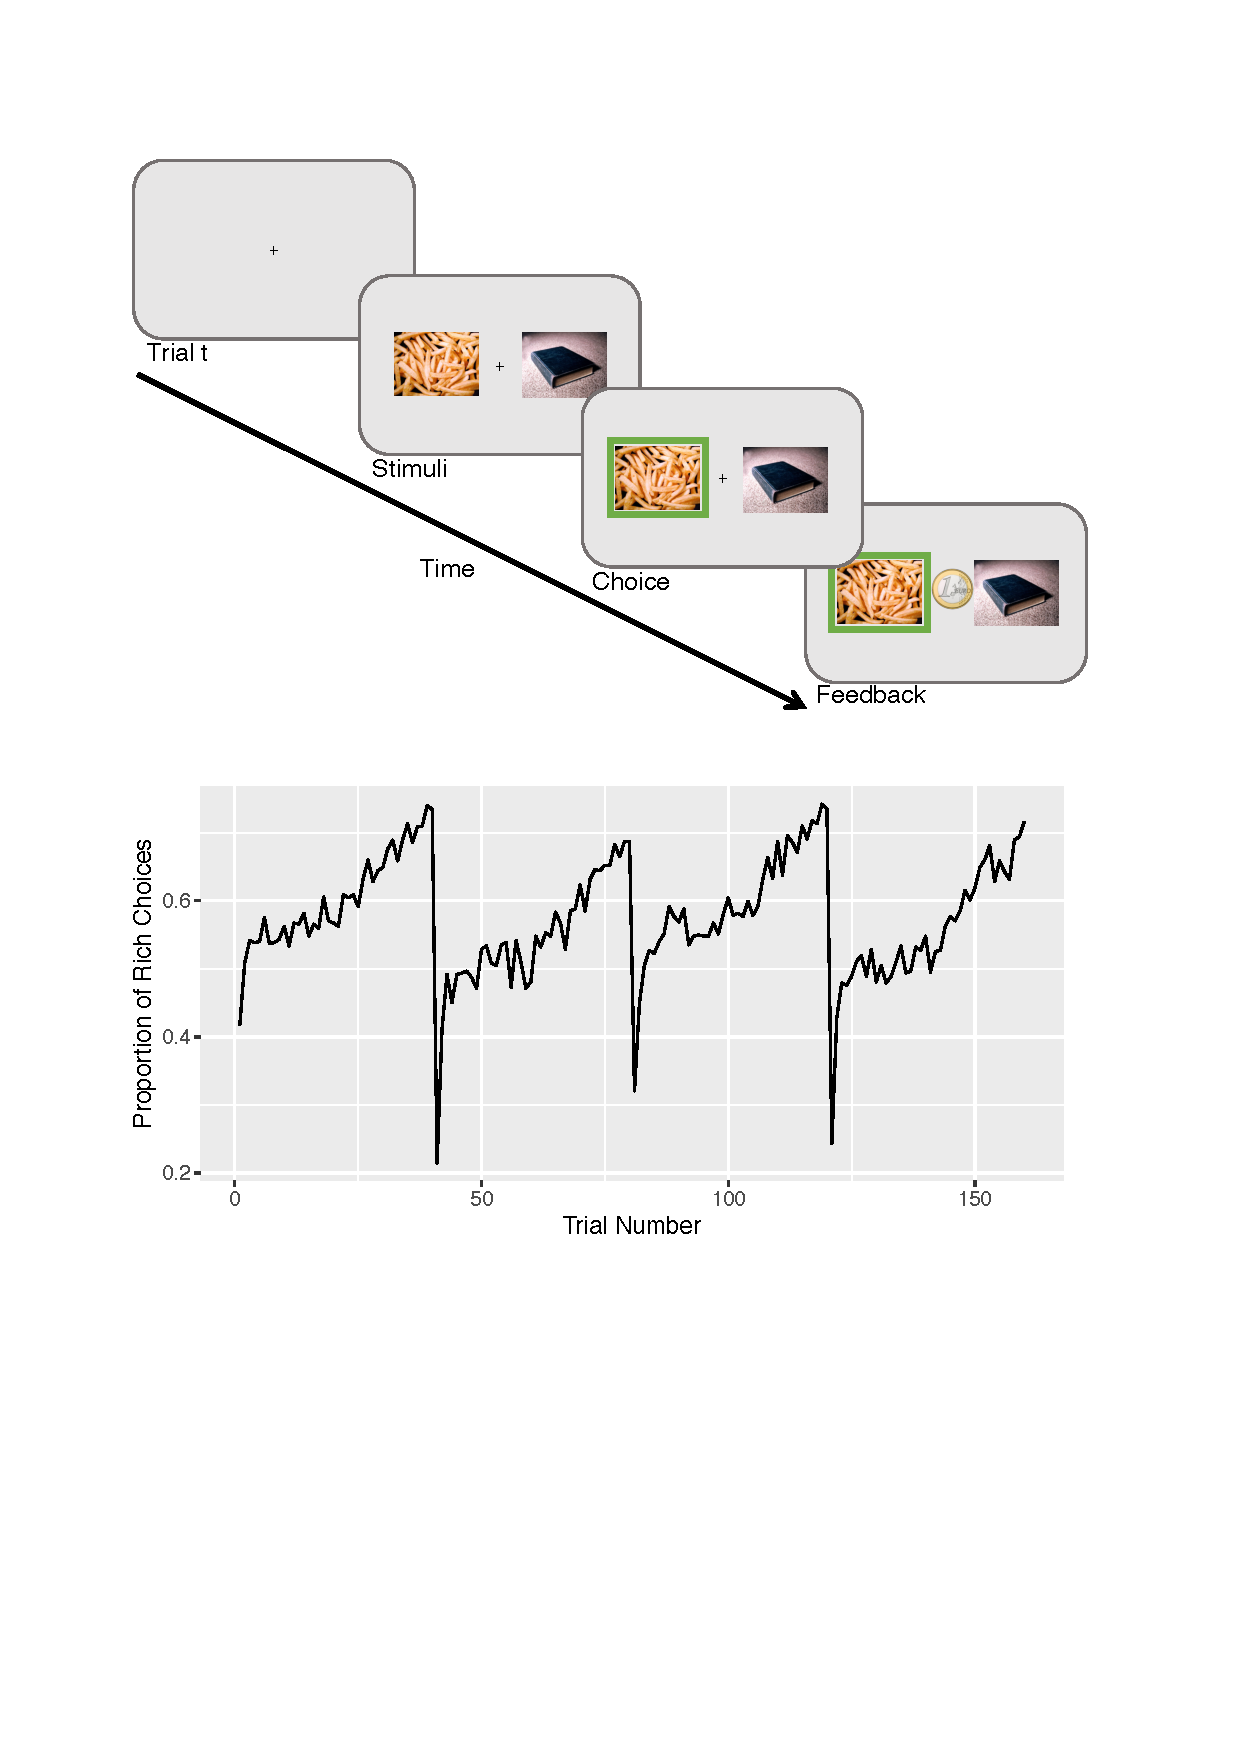
\includegraphics[width=0.85\linewidth]{img/pics/prl_task} 

}

\caption{\textbf{Top.} During the PRL task, participants were presented with two images and had to choose the ``correct'' image based on trial-and-error feedback within 2.5 seconds. A euro coin image was displayed as a reward for correct responses, while a strike-through image of a euro coin served as a punishment for incorrect responses (left or right button press). The PRL task consisted of two blocks of 160 trials each. One block included pairs of food-related and food-unrelated images, while the other block only included food-unrelated images. The figure illustrates a single trial of the PRL task. \textbf{Bottom.} The trial-by-trial proportion of choosing the image with the highest probability of reward in the first epoch is shown for all participants. Initially, when participants have limited knowledge of the contingencies, the proportion of positive rewards is at chance level. However, as they engage in trial-and-error learning, their action selection improves, leading to enhanced performance and increased rewards. Following a context switch, there is an abrupt decline in performance, which is then followed by a gradual recovery that eventually levels off. It is worth noting that in this particular experiment, ``correct choices'' were rewarded positively only 70\% of the time, thus establishing an upper limit of 0.7 on the plateau. Each session comprised 160 trials and included three context switches.}\label{fig:prl-task}
\end{figure}

The stimuli shown in each trial were randomly selected from sets of food-related and food-unrelated images. All images used in the study were obtained from the International Affective Picture System (IAPS) database (Lang, Bradley, Cuthbert, et al., 1997) -- for details, see the SI.

\hypertarget{data-analysis}{%
\subsection{Data analysis}\label{data-analysis}}

To analyze the temporal dynamics of the two-choice decision-making in the PRL task, we employed a hierarchical reinforcement learning drift diffusion model (RLDDM), as described in Pedersen, Frank, and Biele (2017) and Pedersen and Frank (2020). Cognitive modeling analysis allows us to deconstruct decision-making task performance into its component processes, which can help us identify deviations in the underlying mechanisms that may not be evident in the overall task outcome.

We used a Bayesian approach in our study because estimating RLDDM models is currently only possible using Markov chain Monte Carlo (MCMC) procedures. Additionally, the Bayesian approach prioritizes estimation over hypothesis testing, which helps to overcome the binary nature of decision-making inherent in null hypothesis significance testing (NHST) (Kruschke \& Liddell, 2018). We determined credible effects by examining 95\% credible intervals or assessing the proportion of posterior samples (97.5\%) indicating the direction of the effect.

The RLDDM consists of two key components. The first component describes how reward feedback is used to update value expectations, using a delta learning rule (Rescorla \& Wagner, 1972). The second component describes how an agent uses these expectations to arrive at a decision, using a drift-diffusion model (Ratcliff \& McKoon, 2008). The DDM assumes that evidence for each option accumulates stochastically on each trial, until a decision is made (for details, see SI).

The RLDDM has six basic parameters:

\begin{itemize}
\tightlist
\item
  \(\alpha^+\) and \(\alpha^-\): These parameters quantify the learning rate in the Rescorla-Wagner delta learning rule. A higher learning rate results in rapid adaptation to reward expectations, while a lower learning rate results in slow adaptation. The parameter \(\alpha^+\) is computed from reinforcements, whereas \(\alpha^-\) is computed from punishments.
\item
  \(v\): The drift rate is the average speed of evidence accumulation toward one decision.
\item
  \(a\): The decision boundary is the distance between two decision thresholds. An increase of \(a\) increases the evidence needed to make a decision. The increase of \(a\) leads to a slower but more accurate decision; a decrease in a results in a faster but error-prone decision.
\item
  \(t\): The non-decision time is the time spent for stimuli encoding or motor execution (i.e., time not used for evidence accumulation).
\item
  \(z\): The starting point parameter captures a potential initial bias toward one or the other boundary in absence of any stimulus evidence.
\end{itemize}

To assess the presence of context-dependent learning, we conditioned the model's parameters on two contexts: disorder-related choices and disorder-unrelated choices. This allowed us to examine how the model's parameters varied in response to these different contextual conditions.

\hypertarget{results}{%
\section{Results}\label{results}}

\hypertarget{models-selection}{%
\subsection{Models selection}\label{models-selection}}

We evaluated context-dependent learning by comparing several RLDDM models that differed in how they conditioned the model's parameters on group (R-AN, HC, RI) and context (disorder-related choices and disorder-unrelated choices). We used the Deviance Information Criterion (DIC) to balance model fit and complexity, and selected the model with the lowest DIC as the best trade-off. The following RLDDM models were examined. Model M1: Standard RLDDM without conditioning. DIC = 39879.444. Model M2: Separate learning rates for positive and negative reinforcements. DIC = 39124.890 Model M3: Group-based \(\alpha^+\) and \(\alpha^-\) parameters. DIC = 39194.763. Model M4: Group and context-based \(\alpha^+\) and \(\alpha^-\) parameters. DIC = 38197.467. Model M5: Group and context-based \(\alpha^+\), \(\alpha^-\), and \(a\) parameters. DIC = 36427.448. Model M6: Group and context-based \(\alpha^+\), \(\alpha^-\), \(a\), and drift rate (\(v\)) parameters. DIC = 36185.146. Model M7: Group and context-based \(\alpha^+\), \(\alpha^-\), \(a\), \(v\), and non-decision time (\(t\)) parameters. DIC = 34904.053. Model M8: Group and context-based \(\alpha^+\), \(\alpha^-\), \(a\), \(v\), \(t\), and starting point (\(z\)) parameters. DIC = 34917.762. Among the evaluated models, Model M7 had the lowest DIC, indicating the best trade-off between goodness of fit and model complexity. In Model M7, the parameters \(\alpha^+\), \(\alpha^-\), \(a\), \(v\), and \(t\) (excluding \(z\)) were conditioned on both the group and the context.

\hypertarget{modelling-results}{%
\subsection{Modelling results}\label{modelling-results}}

Model M7 was estimated using 15,000 iterations, with a burn-in period of 5,000 iterations. Convergence of the Bayesian estimation was evaluated using the Gelman-Rubin statistic. The \(\hat{R}\) values for all parameters in Model M7 were below 1.1, indicating that the model converged well. Collinearity and posterior predictive checks were also used to evaluate model validity (see SI).

To investigate the impact of disorder-related versus disorder-unrelated information on RL learning, we compared the posterior estimates of the RLDDM parameters of Model M7 between the two conditions (see Table 1).

\begin{longtable}[]{@{}
  >{\raggedright\arraybackslash}p{(\columnwidth - 10\tabcolsep) * \real{0.0943}}
  >{\raggedright\arraybackslash}p{(\columnwidth - 10\tabcolsep) * \real{0.1887}}
  >{\raggedright\arraybackslash}p{(\columnwidth - 10\tabcolsep) * \real{0.2642}}
  >{\raggedright\arraybackslash}p{(\columnwidth - 10\tabcolsep) * \real{0.2075}}
  >{\raggedright\arraybackslash}p{(\columnwidth - 10\tabcolsep) * \real{0.1132}}
  >{\raggedright\arraybackslash}p{(\columnwidth - 10\tabcolsep) * \real{0.1321}}@{}}
\caption{Posterior Parameter Estimates of DDMRL Model M7 by Group (R-AN, HC, RI) and Context of PRL Choice (disorder-related vs.~disorder-unrelated information). The learning rates (\(\alpha\)) are shown on a logit scale. The probability (\(p\)) describes the Bayesian test that the posterior estimate of the parameter in the disorder-related context is greater than the posterior estimate of the parameter in the disorder-unrelated context. Standard deviations are provided in parentheses.}\tabularnewline
\toprule\noalign{}
\begin{minipage}[b]{\linewidth}\raggedright
Group
\end{minipage} & \begin{minipage}[b]{\linewidth}\raggedright
Par.
\end{minipage} & \begin{minipage}[b]{\linewidth}\raggedright
Neutral choice
\end{minipage} & \begin{minipage}[b]{\linewidth}\raggedright
Food choice
\end{minipage} & \begin{minipage}[b]{\linewidth}\raggedright
\(p\)
\end{minipage} & \begin{minipage}[b]{\linewidth}\raggedright
Cohen's \(d\)
\end{minipage} \\
\midrule\noalign{}
\endfirsthead
\toprule\noalign{}
\begin{minipage}[b]{\linewidth}\raggedright
Group
\end{minipage} & \begin{minipage}[b]{\linewidth}\raggedright
Par.
\end{minipage} & \begin{minipage}[b]{\linewidth}\raggedright
Neutral choice
\end{minipage} & \begin{minipage}[b]{\linewidth}\raggedright
Food choice
\end{minipage} & \begin{minipage}[b]{\linewidth}\raggedright
\(p\)
\end{minipage} & \begin{minipage}[b]{\linewidth}\raggedright
Cohen's \(d\)
\end{minipage} \\
\midrule\noalign{}
\endhead
\bottomrule\noalign{}
\endlastfoot
R-AN & a & 1.273 (0.039) & 1.442 (0.040) & 0.0013 & 0.802 \\
R-AN & v & 1.403 (0.320) & 1.776 (0.342) & 0.7907 & 0.190 \\
R-AN & t & 0.188 (0.011) & 0.174 (0.011) & 0.8311 & -0.253 \\
R-AN & \(\alpha^-\) & 1.815 (1.081) & 0.738 (1.096) & 0.2349 & -0.432 \\
R-AN & \(\alpha^+\) & 1.006 (0.899) & -1.786 (0.756) & 0.0098 & -1.206 \\
HC & a & 1.222 (0.033) & 1.314 (0.034) & 0.0256 & 0.474 \\
HC & v & 2.157 (0.265) & 1.790 (0.263) & 0.1606 & -0.358 \\
HC & t & 0.183 (0.009) & 0.172 (0.009) & 0.8228 & -0.280 \\
HC & \(\alpha^-\) & 2.780 (0.874) & 3.442 (0.980) & 0.6993 & 0.298 \\
HC & \(\alpha^+\) & 1.198 (0.680) & 1.326 (0.700) & 0.5544 & 0.071 \\
RI & a & 1.245 (0.041) & 1.316 (0.039) & 0.1026 & 0.403 \\
RI & v & 2.197 (0.322) & 1.849 (0.307) & 0.2133 & -0.381 \\
RI & t & 0.188 (0.011) & 0.186 (0.011) & 0.5462 & 0.166 \\
RI & \(\alpha^-\) & 2.857 (1.067) & 2.904 (1.062) & 0.5101 & 0.015 \\
RI & \(\alpha^+\) & 1.573 (0.847) & 0.739 (0.752) & 0.2247 & -0.438 \\
\end{longtable}

Let's first consider the evidence of context-dependent learning from within-group comparisons (Figure \ref{fig:alpha-param}, panel B). We found that individuals in the R-AN group had a reduced learning rate from rewards for disorder-related choices, compared to disorder-unrelated choices (Cohen's \(d\) = -1.206, \(p\) = 0.0098). However, no credible difference was found in the learning rate between disorder-related and disorder-unrelated choices in the HC (\(p\) = 0.5544) or RI (\(p\) = 0.2247) groups. We found no credible difference in the learning rate from punishments between disorder-related and disorder-unrelated choices for any of the R-AN (\(p\) = 0.2349), HC (\(p\) = 0.6993), and RI (\(p\) = 0.5101) groups. Moreover, we found that individuals with R-AN showed a higher decision threshold for disorder-related choices compared to disorder-unrelated choices (Cohen's \(d\) = 0.802, \(p\) = 0.0013) -- Figure \ref{fig:a-param}, panel B.



\begin{figure}

{\centering 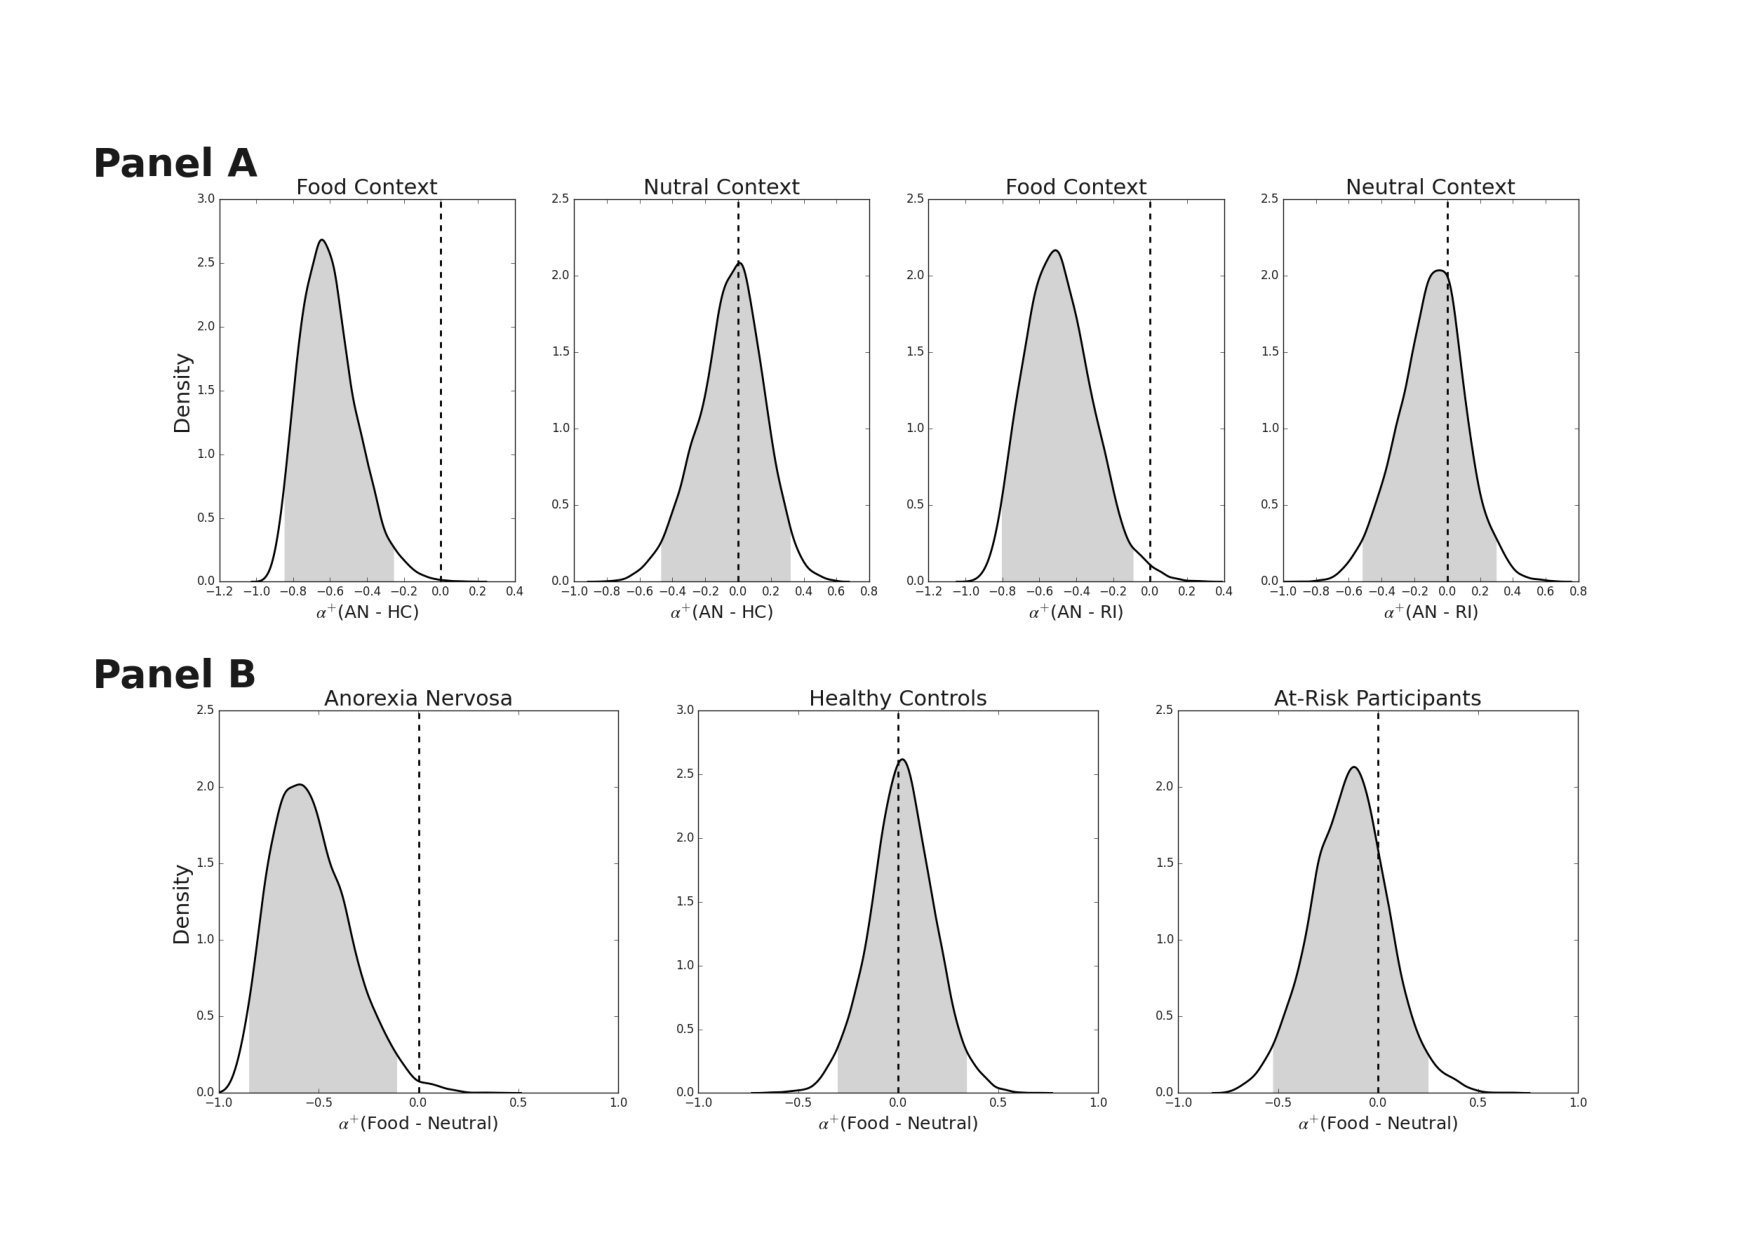
\includegraphics[width=0.99\linewidth]{img/pics/alpha_pos_param} 

}

\caption{\textbf{Panel A.} Plots of the posterior distribution of the group effects (AN - HC; AN - RI) for parameter \(\alpha^+\) of the DDMRL, for disorder-related choices (Food context) and disorder-unrelated (Neutral context) choices. \textbf{Panel B.} Plots of the posterior distribution of the within-group effects (\(\alpha^+_{food} - \alpha^+_{neutral}\)) across the three groups of participants.}\label{fig:alpha-param}
\end{figure}



\begin{figure}

{\centering 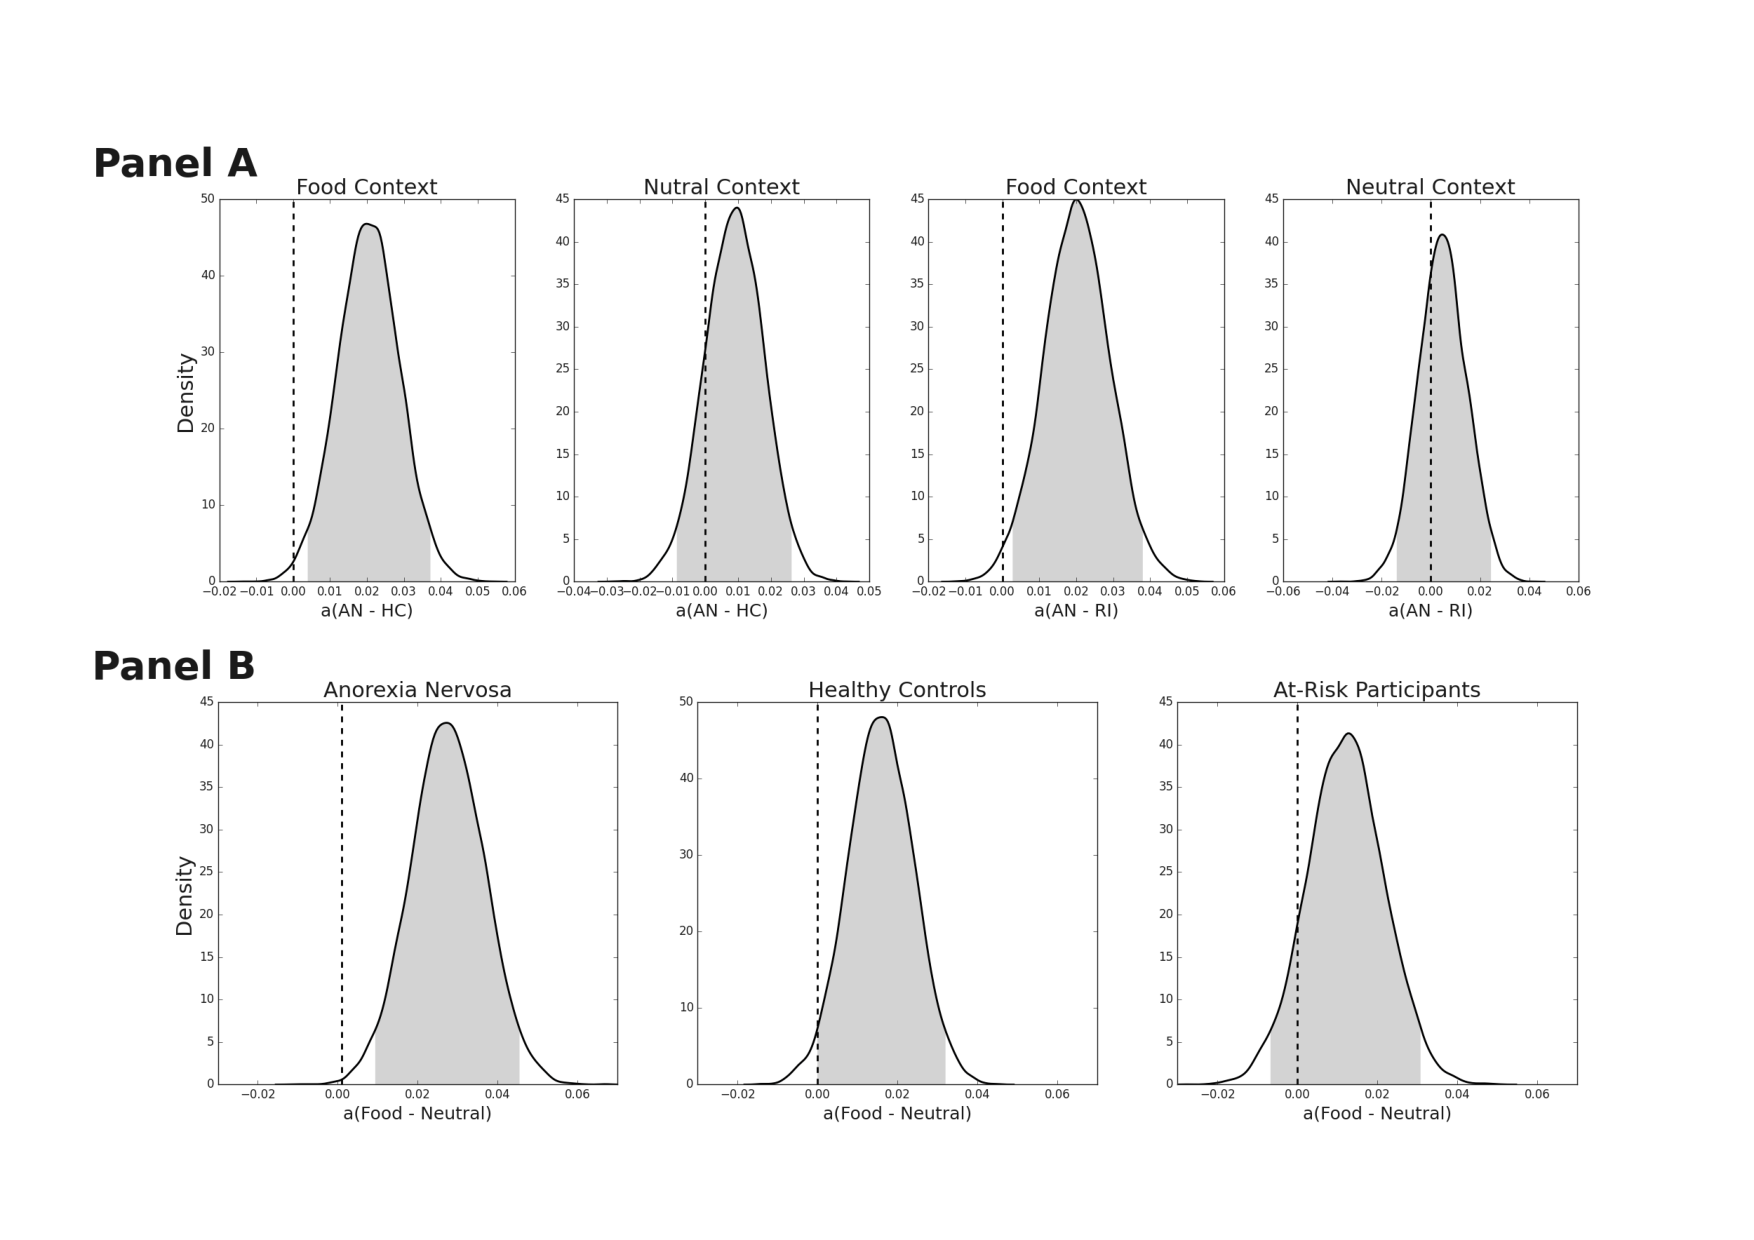
\includegraphics[width=0.99\linewidth]{img/pics/a_param} 

}

\caption{\textbf{Panel A.} Plots of the posterior distribution of the group effects (AN - HC; AN - RI) for parameter \(a\) of the DDMRL, for disorder-related choices (Food context) and disorder-unrelated (Neutral context) choices. \textbf{Panel B.} Plots of the posterior distribution of the within-group effects (\(a_{food} - a_{neutral}\)) across the three groups of participants.}\label{fig:a-param}
\end{figure}

Further evidence of context-dependent learning emerges from between-groups comparisons. When making disorder-related choices, individuals with R-AN displayed a decreased learning rate from rewards compared to both HC (\(p\) = 0.0009, Cohen's \(d\) = 1.498) and RI (\(p\) = 0.0085, Cohen's \(d\) = 1.209) -- Figure \ref{fig:alpha-param}, panel A. In contrast, no credible difference in the learning rate from rewards was found between R-AN and HC (\(p\) = 0.4325), as well as between R-AN and RI (\(p\) = 0.3232), for choices unrelated to disorder information. Individuals with R-AN showed a higher decision threshold for disorder-related choices compared to both HC (Cohen's \(d\) = -0.622, \(p\) = 0.0068) and RI (Cohen's \(d\) = -0.454, \(p\) = 0.0118) participants, whereas no credible group differences were found for disorder-unrelated choices (Figure \ref{fig:a-param}, panel A). Finally, no credible differences were found, for both within-group and between-group comparisons, regarding the drift rate (\(\nu\)) and the non-decision time parameters (\(t\)).

\hypertarget{preferential-choices}{%
\subsection{Preferential choices}\label{preferential-choices}}

To investigate the presence of a bias against food choices in individuals with R-AN during the PRL task, regardless of their past action-outcome history, we analyzed the frequency of food choices in PRL blocks where a food image was paired with a neutral image. Our results show that the AN-R group did not exhibit a bias against the food image, with a proportion of food choices estimated at 0.49, 95\% CI {[}0.46, 0.51{]}. Furthermore, there were no credible differences in food choices between the R-AN group and the HC group (contrast R-AN - HC = -0.007, 95\% CI {[}-0.037, 0.024{]}) or between the R-AN group and the RI group (contrast R-AN - RI = 0.013, 95\% CI {[}-0.019, 0.046{]}).

\hypertarget{comorbidity}{%
\subsection{Comorbidity}\label{comorbidity}}

To examine the potential impact of comorbidity and medication status on the present results, we compared R-AN participants who had diagnosed comorbidities (45\% of the sample) and those without any comorbid conditions using Model M7. We did not find any credible differences in parameters between the two groups. Specifically, when considering the disorder-related context, the parameter differences were as follows: \(\Delta \alpha^-\) = 2.614, 95\% CI {[}-3.173, 8.364{]}; \(\Delta \alpha^+\) = -0.635, 95\% CI {[}-4.301, 2.449{]}; \(\Delta a\) = -0.034, 95\% CI {[}-0.188, 0.124{]}; \(\Delta v\) = 0.230, 95\% CI {[}-1.203, 1.586{]}; \(\Delta t\) = 0.002, 95\% CI {[}-0.050, 0.055{]}. Similarly, for the disorder-unrelated context, the parameter differences were: \(\Delta \alpha^-\) = -0.768, 95\% CI {[}-6.570, 4.401{]}; \(\Delta \alpha^+\) = -1.739, 95\% CI {[}-6.184, 1.654{]}; \(\Delta a\) = -0.126, 95\% CI {[}-0.281, 0.025{]}; \(\Delta v\) = 0.744, 95\% CI {[}-0.453, 1.886{]}; \(\Delta t\) = -0.003, 95\% CI {[}-0.057, 0.052{]}. The correlation between comorbidity and medication was 0.78.

\hypertarget{discussion}{%
\subsection{Discussion}\label{discussion}}

Our study reveal a context-dependent learning asymmetry in individuals with R-AN, specifically in the positive learning rate (\(\alpha^+\)). This asymmetry is evident when comparing their performance in the PRL task for disorder-related choices versus disorder-unrelated choices. Notably, this difference is not observed in the two control groups.

The presence of context-dependent learning asymmetry is also supported by between-group comparisons. Individuals with R-AN exhibited lower learning rates (\(\alpha^+\)) compared to the HC and RI group. However, these differences were observed only for disorder-related choices. In contrast, no credible differences in learning rates were found among the three groups for choices unrelated to the disorder.

Support for context-dependent learning in R-AN is also provided by the DDM parameters of the RLDDM model. Specifically, we observed that the R-AN group exhibited a higher decision threshold (parameter ``a'' in the RLDDM model) compared to the HC and RI groups, but this difference was only evident in the context of disorder-related choices. Additionally, individuals with R-AN exhibited a higher decision threshold for disorder-related choices compared to disorder-unrelated choices, which was not seen in the HC and RI groups. Overall, these results suggest that individuals with R-AN tended to display a more cautious or conservative decision-making behavior in relation to choices related to the disorder (see also Caudek, Sica, Cerea, Colpizzi, \& Stendardi, 2021; Schiff, Testa, Rusconi, Angeli, \& Mapelli, 2021). We did not find any credible contextual effects or group differences for the parameters \(\nu\) and \(t\).

The analysis of preferential choices supports the conclusion that the learning performance asymmetry observed in individuals with R-AN is not due to a preferential selection of the disorder-unrelated image during the learning task. Additionally, our analysis examining the relationship between the model's parameters and the presence of comorbidities indicates that the learning performance asymmetry in individuals with R-AN cannot be attributed to comorbid conditions.

\hypertarget{general-discussion}{%
\section{General discussion}\label{general-discussion}}

In this study, we investigated reinforcement learning using a behavioral paradigm that included two distinct learning contexts: one involving choices related to food and the other involving choices unrelated to food. We compared the performance of patients with R-AN to age-, gender-, and education-matched healthy controls, as well as healthy controls at-risk of developing eating disorders. Consistent with our hypotheses, our findings revealed a lower learning rate in the disorder-related context for individuals with R-AN, whereas both healthy participants and at-risk individuals learned equally well in both contexts.

In PRL tasks, a participant's performance can be influenced by two potential factors. First, there may be a learning impairment, where participants struggle to accurately update the value of the stimuli. Second, there may be a decision impairment, where participants may still select the wrong stimulus despite having intact learning processes. Our results show that individuals with R-AN may struggle with both accurately updating the value of disorder-related stimuli and making appropriate decisions based on this information. However, we did not observe similar impairments in decision making for disorder-unrelated choices. These findings provide evidence for context-dependent learning in individuals with R-AN, where the inclusion of disorder-related information negatively impacts their RL performance. It is important to note that this effect is specific to the disorder-related context and does not suggest a generalized RL deficit in individuals with R-AN. Thus, our results challenge the notion of a domain-general RL mechanism impairment in this population (see Bernardoni et al., 2021).

Previous studies have demonstrated that reward and punishment processing in individuals with AN is influenced by stimulus properties and contextual factors. For instance, predictable and controllable behaviors such as calorie counting or purging are often perceived as rewarding, providing individuals with a sense of control and accomplishment. Conversely, unpredictable and uncontrollable situations, such as social outcomes, can be perceived as punishing, leading to heightened anxiety and distress (Haynos et al., 2020). While previous studies have predominantly examined the impact of context on the subjective value attributed to experiences in AN, our study expands on this research by demonstrating that context plays a crucial role in the actual learning process itself (Heald et al., 2023). This goes beyond solely influencing subjective value and provides valuable insights into how reward and punishment processing operates in AN.

Other recent studies have focused on investigating context-specific learning in eating disorders. One task specifically designed for this purpose is the two-step Markov decision task, which distinguishes between automatic or habitual (model-free) learning and controlled or goal-directed (model-based) learning. For instance, studies conducted by Foerde et al. (2021) and Onysk and Seriès (2022) employed similar experiments using the two-step task paradigm. Foerde et al. (2021) compared a monetary two-step task and a food-related two-step task, while Onysk and Seriès (2022) utilized stimuli unrelated to food or body images (i.e., pirate ships and treasure chests) with rewards associated with body image dissatisfaction. The results of these studies consistently demonstrated that individuals with AN tend to exhibit a stronger inclination towards habitual control over goal-directed control across different domains compared to healthy controls. However, these studies did not identify significant differences in learning rates based on context or between AN patients and healthy controls. In contrast, the present study reveals that, in individuals with R-AN, the learning process \emph{per se} (i.e., the learning rates) can be influenced by contextual (disorder-related) information, even when contextual information is not directly relevant to the task outcome.

The finding that individuals with R-AN demonstrated a conservative learning rate specifically for rewards in response to disorder-related context, but not for punishments, supports a neurobiological model suggesting that AN symptoms are maintained by diminished responses to rewarding stimuli and exaggerated responses to aversive stimuli, potentially due to an overreliance on cognitive control brain circuitry (Wierenga et al., 2014). A study by Bernardoni et al. (2018), which used a PRL task with disorder-unrelated stimuli, revealed increased learning rates specifically after punishments in AN. This study suggested that AN individuals, when faced with negative feedback, tend to critically reassess their beliefs more quickly than healthy controls (HCs), leading them to base decisions on more recent experiences. Such inclination may be linked to pre-existing harm-avoidant traits in AN patients, characterized by a reduced tolerance for negative outcomes. Considering these factors, we speculate that the lack of contextual effect on negative learning rates in our study may arise from a trade-off between the conservative learning induced by disorder-related cues and the increased learning rate observed after punishment.

The hypothesis proposing that reinforcement learning (RL) anomalies in individuals with anorexia nervosa (AN) may be influenced by contextual factors carries significant implications for treatment strategies. Currently, Cognitive Remediation Therapy (CRT) is utilized to address cognitive inflexibility in AN and other eating disorders. CRT involves cognitive exercises and behavioral interventions aimed at improving central coherence abilities, reducing cognitive and behavioral inflexibility, and enhancing thinking style comprehension (Tchanturia, Davies, Reeder, \& Wykes, 2010). A key aspect of CRT is to avoid addressing symptom-related themes and instead utilize neutral stimuli in cognitive and behavioral exercises. This approach aims to establish a therapeutic alliance and reduce drop-out rates, particularly among individuals with AN. However, recent evidence suggests that CRT may not consistently improve central coherence abilities, cognitive flexibility, or symptoms associated with eating disorders (Hagan, Christensen, \& Forbush, 2020; Tchanturia, Giombini, Leppanen, \& Kinnaird, 2017). In response to these findings, Trapp, Heid, Röder, Wimmer, and Hajak (2022) propose modifications to address practical challenges encountered in the application of CRT. They question the use of neutral stimuli and draw support from Beck's cognitive theory of depression (Beck \& Alford, 2009). This proposition aligns with the hypothesis of our study. If further studies consistently demonstrate that maladaptive RL is context-dependent, it would necessitate a shift in intervention approaches.

There are few important limitations and questions for future research. 1) One aspect to consider is the use of symbolic rewards and punishments in our study, represented by images of a one euro coin and a barred representation of a one euro coin, respectively. These rewards and punishments were merely symbolic, and it is unclear how the use of concrete, non-symbolic rewards and punishments would impact the findings. Additionally, the subjective value of one euro, or the loss of one euro, may vary among participants. Therefore, future studies could aim to determine the equivalence of subjective values for rewards and punishments to enhance the understanding of the underlying processes. 2) Our study only included individuals with R-AN who were not in the most severe stage of the illness, as they were recruited from a center for voluntary medical and psychological support. We did not examine R-AN patients who require hospitalization due to the life-threatening nature of their illness. It is possible that at the later stages of the illness, associative learning abilities, which were preserved in the present sample under neutral conditions, may become impaired. Therefore, investigating the impact of illness severity on context-dependent learning in R-AN patients is an important avenue for future research. 3) While we observed no difference in the choice behavior of R-AN patients, as measured by the relative frequency of image choices, when selecting between a neutral image and a food image, we did find a slower learning rate and lower decision threshold for R-AN patients compared to healthy controls in the RLDDM model when compared to choosing between two neutral images. It is possible that the higher ``salience'' of food images compared to neutral images could be better captured by other measures, such as fixation length or the number of fixations, rather than solely relying on the relative frequency of image choices. This warrants further exploration in future studies. 4) It is worth noting that our study excluded women under the age of 18. However, this age range is a critical period as the onset of AN during this stage may have a more profound impact on associative learning, given the ongoing cognitive development and less-developed protective factors. Therefore, future studies should take into consideration the inclusion of participants in this age range to better understand the influence of context-dependent learning in R-AN.

\newpage

\hypertarget{references}{%
\section{References}\label{references}}

\hypertarget{refs}{}
\begin{CSLReferences}{1}{0}
\leavevmode\vadjust pre{\hypertarget{ref-dsm5tr}{}}%
American Psychiatric Association. (2022). \emph{{Diagnostic and Statistical Manual of Mental Disorders}} (5th ed., Text Revision). Arlington, VA: {American Psychiatric Publishing}.

\leavevmode\vadjust pre{\hypertarget{ref-atwood2020systematic}{}}%
Atwood, M. E., \& Friedman, A. (2020). A systematic review of enhanced cognitive behavioral therapy (CBT-e) for eating disorders. \emph{International Journal of Eating Disorders}, \emph{53}(3), 311--330.

\leavevmode\vadjust pre{\hypertarget{ref-bartholdy2016systematic}{}}%
Bartholdy, S., Dalton, B., O'Daly, O. G., Campbell, I. C., \& Schmidt, U. (2016). A systematic review of the relationship between eating, weight and inhibitory control using the stop signal task. \emph{Neuroscience \& Biobehavioral Reviews}, \emph{64}, 35--62.

\leavevmode\vadjust pre{\hypertarget{ref-beck2009depression}{}}%
Beck, A. T., \& Alford, B. A. (2009). \emph{Depression: Causes and treatment}. University of Pennsylvania Press.

\leavevmode\vadjust pre{\hypertarget{ref-bernardoni_altered_2018}{}}%
Bernardoni, F., Geisler, D., King, J. A., Javadi, A.-H., Ritschel, F., Murr, J., \ldots{} Ehrlich, S. (2018). Altered medial frontal feedback learning signals in {Anorexia} {Nervosa}. \emph{Biological Psychiatry}, \emph{83}(3), 235--243.

\leavevmode\vadjust pre{\hypertarget{ref-bernardoni2021more}{}}%
Bernardoni, F., King, J. A., Geisler, D., Ritschel, F., Schwoebel, S., Reiter, A. M., \ldots{} Ehrlich, S. (2021). More by stick than by carrot: A reinforcement learning style rooted in the medial frontal cortex in anorexia nervosa. \emph{Journal of Abnormal Psychology}, \emph{130}(7), 736--747.

\leavevmode\vadjust pre{\hypertarget{ref-bischoff2013altered}{}}%
Bischoff-Grethe, A., McCurdy, D., Grenesko-Stevens, E., Irvine, L. E. Z., Wagner, A., Yau, W.-Y. W., et al.others. (2013). Altered brain response to reward and punishment in adolescents with anorexia nervosa. \emph{Psychiatry Research: Neuroimaging}, \emph{214}(3), 331--340.

\leavevmode\vadjust pre{\hypertarget{ref-caudek2021susceptibility}{}}%
Caudek, C., Sica, C., Cerea, S., Colpizzi, I., \& Stendardi, D. (2021). Susceptibility to eating disorders is associated with cognitive inflexibility in female university students. \emph{Journal of Behavioral and Cognitive Therapy}, \emph{31}(4), 317--328.

\leavevmode\vadjust pre{\hypertarget{ref-chang2021early}{}}%
Chang, P. G., Delgadillo, J., \& Waller, G. (2021). Early response to psychological treatment for eating disorders: A systematic review and meta-analysis. \emph{Clinical Psychology Review}, \emph{86}, 102032.

\leavevmode\vadjust pre{\hypertarget{ref-dottiandlazzari1998}{}}%
Dotti, A., \& Lazzari, R. (1998). Validation and reliability of the italian {EAT-26}. \emph{Eating and Weight Disorders-Studies on Anorexia, Bulimia and Obesity}, \emph{3}(4), 188--194.

\leavevmode\vadjust pre{\hypertarget{ref-DowsonandHenderson2001}{}}%
Dowson, J., \& Henderson, L. (2001). The validity of a short version of the {Body Shape Questionnaire}. \emph{Psychiatry Research}, \emph{102}(3), 263--271.

\leavevmode\vadjust pre{\hypertarget{ref-fladung2013role}{}}%
Fladung, A.-K., Schulze, U. M., Schöll, F., Bauer, K., \& Groen, G. (2013). Role of the ventral striatum in developing anorexia nervosa. \emph{Translational Psychiatry}, \emph{3}(10), e315--e315.

\leavevmode\vadjust pre{\hypertarget{ref-foerde2021deficient}{}}%
Foerde, K., Daw, N. D., Rufin, T., Walsh, B. T., Shohamy, D., \& Steinglass, J. E. (2021). Deficient goal-directed control in a population characterized by extreme goal pursuit. \emph{Journal of Cognitive Neuroscience}, \emph{33}(3), 463--481.

\leavevmode\vadjust pre{\hypertarget{ref-frost1990dimensions}{}}%
Frost, R. O., Marten, P., Lahart, C., \& Rosenblate, R. (1990). The dimensions of perfectionism. \emph{Cognitive Therapy and Research}, \emph{14}(5), 449--468.

\leavevmode\vadjust pre{\hypertarget{ref-galmiche2019prevalence}{}}%
Galmiche, M., Déchelotte, P., Lambert, G., \& Tavolacci, M. P. (2019). Prevalence of eating disorders over the 2000--2018 period: A systematic literature review. \emph{The American Journal of Clinical Nutrition}, \emph{109}(5), 1402--1413.

\leavevmode\vadjust pre{\hypertarget{ref-Garner1991}{}}%
Garner, D. M. (1991). \emph{{Eating Drjorder Inventory-2 Manual}}. Odessa, Fla.: Psychological Assessment Resources.

\leavevmode\vadjust pre{\hypertarget{ref-geisler2017increased}{}}%
Geisler, D., Ritschel, F., King, J. A., Bernardoni, F., Seidel, M., Boehm, I., et al.others. (2017). Increased anterior cingulate cortex response precedes behavioural adaptation in anorexia nervosa. \emph{Scientific Reports}, \emph{7}(1), 42066.

\leavevmode\vadjust pre{\hypertarget{ref-glashouwer2014heightened}{}}%
Glashouwer, K. A., Bloot, L., Veenstra, E. M., Franken, I. H., \& Jong, P. J. de. (2014). Heightened sensitivity to punishment and reward in anorexia nervosa. \emph{Appetite}, \emph{75}, 97--102.

\leavevmode\vadjust pre{\hypertarget{ref-guillaume2015impaired}{}}%
Guillaume, S., Gorwood, P., Jollant, F., Van den Eynde, F., Courtet, P., \& Richard-Devantoy, S. (2015). Impaired decision-making in symptomatic anorexia and bulimia nervosa patients: A meta-analysis. \emph{Psychological Medicine}, \emph{45}(16), 3377--3391.

\leavevmode\vadjust pre{\hypertarget{ref-hagan2020preliminary}{}}%
Hagan, K. E., Christensen, K. A., \& Forbush, K. T. (2020). A preliminary systematic review and meta-analysis of randomized-controlled trials of cognitive remediation therapy for anorexia nervosa. \emph{Eating Behaviors}, \emph{37}, 101391.

\leavevmode\vadjust pre{\hypertarget{ref-harrison2011experimental}{}}%
Harrison, A., Genders, R., Davies, H., Treasure, J., \& Tchanturia, K. (2011). Experimental measurement of the regulation of anger and aggression in women with anorexia nervosa. \emph{Clinical Psychology \& Psychotherapy}, \emph{18}(6), 445--452.

\leavevmode\vadjust pre{\hypertarget{ref-haynos2020moving}{}}%
Haynos, A. F., Lavender, J. M., Nelson, J., Crow, S. J., \& Peterson, C. B. (2020). Moving towards specificity: A systematic review of cue features associated with reward and punishment in anorexia nervosa. \emph{Clinical Psychology Review}, \emph{79}, 101872.

\leavevmode\vadjust pre{\hypertarget{ref-haynos2022beyond}{}}%
Haynos, A. F., Widge, A. S., Anderson, L. M., \& Redish, A. D. (2022). Beyond description and deficits: How computational psychiatry can enhance an understanding of decision-making in anorexia nervosa. \emph{Current Psychiatry Reports}, 1--11.

\leavevmode\vadjust pre{\hypertarget{ref-heald2023contextual}{}}%
Heald, J. B., Lengyel, M., \& Wolpert, D. M. (2023). Contextual inference in learning and memory. \emph{Trends in Cognitive Sciences}.

\leavevmode\vadjust pre{\hypertarget{ref-Hildebrandt2015}{}}%
Hildebrandt, T., Grotzinger, A., Reddan, M., Greif, R., Levy, I., Goodman, W., \& Schiller, D. (2015). \href{https://www.ncbi.nlm.nih.gov/pubmed/26131915}{{Testing the disgust conditioning theory of food-avoidance in adolescents with recent onset anorexia nervosa}}. \emph{Behaviour Research and Therapy}, \emph{71}, 131--138.

\leavevmode\vadjust pre{\hypertarget{ref-hildebrandt2018evidence}{}}%
Hildebrandt, T., Schulz, K., Schiller, D., Heywood, A., Goodman, W., \& Sysko, R. (2018). Evidence of prefrontal hyperactivation to food-cue reversal learning in adolescents with anorexia nervosa. \emph{Behaviour Research and Therapy}, \emph{111}, 36--43.

\leavevmode\vadjust pre{\hypertarget{ref-jappe2011heightened}{}}%
Jappe, L. M., Frank, G. K., Shott, M. E., Rollin, M. D., Pryor, T., Hagman, J. O., \ldots{} Davis, E. (2011). Heightened sensitivity to reward and punishment in anorexia nervosa. \emph{International Journal of Eating Disorders}, \emph{44}(4), 317--324.

\leavevmode\vadjust pre{\hypertarget{ref-jonker2022punishment}{}}%
Jonker, N. C., Glashouwer, K. A., \& Jong, P. J. de. (2022). Punishment sensitivity and the persistence of anorexia nervosa: High punishment sensitivity is related to a less favorable course of anorexia nervosa. \emph{International Journal of Eating Disorders}, \emph{55}(5), 697--702.

\leavevmode\vadjust pre{\hypertarget{ref-keating2010theoretical}{}}%
Keating, C. (2010). Theoretical perspective on anorexia nervosa: The conflict of reward. \emph{Neuroscience \& Biobehavioral Reviews}, \emph{34}(1), 73--79.

\leavevmode\vadjust pre{\hypertarget{ref-keating2012reward}{}}%
Keating, C., Tilbrook, A. J., Rossell, S. L., Enticott, P. G., \& Fitzgerald, P. B. (2012). Reward processing in anorexia nervosa. \emph{Neuropsychologia}, \emph{50}(5), 567--575.

\leavevmode\vadjust pre{\hypertarget{ref-kruschke_bayesian_2018}{}}%
Kruschke, J. K., \& Liddell, T. M. (2018). Bayesian data analysis for newcomers. \emph{Psychonomic Bulletin \& Review}, \emph{25}(1), 155--177.

\leavevmode\vadjust pre{\hypertarget{ref-lang1997international}{}}%
Lang, P. J., Bradley, M. M., Cuthbert, B. N., et al. (1997). International affective picture system (IAPS): Technical manual and affective ratings. \emph{NIMH Center for the Study of Emotion and Attention}, \emph{1}(39-58), 3.

\leavevmode\vadjust pre{\hypertarget{ref-linardon2017empirical}{}}%
Linardon, J., Fairburn, C. G., Fitzsimmons-Craft, E. E., Wilfley, D. E., \& Brennan, L. (2017). The empirical status of the third-wave behaviour therapies for the treatment of eating disorders: A systematic review. \emph{Clinical Psychology Review}, \emph{58}, 125--140.

\leavevmode\vadjust pre{\hypertarget{ref-Lovibond1995}{}}%
Lovibond, P. F., \& Lovibond, S. H. (1995). {The structure of negative emotional states: Comparison of the Depression Anxiety Stress Scales (DASS) with the Beck Depression and Anxiety Inventories}. \emph{Behaviour Research and Therapy}, \emph{33}(3), 335--343.

\leavevmode\vadjust pre{\hypertarget{ref-MattickandClarke1998}{}}%
Mattick, R. P., \& Clarke, J. C. (1998). Development and validation of measures of social phobia scrutiny fear and social interaction anxiety. \emph{Behaviour Research and Therapy}, \emph{36}(4), 455--470.

\leavevmode\vadjust pre{\hypertarget{ref-matton2013punishment}{}}%
Matton, A., Goossens, L., Braet, C., \& Vervaet, M. (2013). Punishment and reward sensitivity: Are naturally occurring clusters in these traits related to eating and weight problems in adolescents? \emph{European Eating Disorders Review}, \emph{21}(3), 184--194.

\leavevmode\vadjust pre{\hypertarget{ref-monteleone2017altered}{}}%
Monteleone, A. M., Monteleone, P., Esposito, F., Prinster, A., Volpe, U., Cantone, E., et al.others. (2017). Altered processing of rewarding and aversive basic taste stimuli in symptomatic women with anorexia nervosa and bulimia nervosa: An fMRI study. \emph{Journal of Psychiatric Research}, \emph{90}, 94--101.

\leavevmode\vadjust pre{\hypertarget{ref-o2015reward}{}}%
O'Hara, C. B., Campbell, I. C., \& Schmidt, U. (2015). A reward-centred model of anorexia nervosa: A focussed narrative review of the neurological and psychophysiological literature. \emph{Neuroscience \& Biobehavioral Reviews}, \emph{52}, 131--152.

\leavevmode\vadjust pre{\hypertarget{ref-onysk2022effect}{}}%
Onysk, J., \& Seriès, P. (2022). The effect of body image dissatisfaction on goal-directed decision making in a population marked by negative appearance beliefs and disordered eating. \emph{Plos One}, \emph{17}(11), e0276750.

\leavevmode\vadjust pre{\hypertarget{ref-pedersen2020simultaneous}{}}%
Pedersen, M. L., \& Frank, M. J. (2020). Simultaneous hierarchical bayesian parameter estimation for reinforcement learning and drift diffusion models: A tutorial and links to neural data. \emph{Computational Brain \& Behavior}, \emph{3}, 458--471.

\leavevmode\vadjust pre{\hypertarget{ref-pedersen2017drift}{}}%
Pedersen, M. L., Frank, M. J., \& Biele, G. (2017). The drift diffusion model as the choice rule in reinforcement learning. \emph{Psychonomic Bulletin \& Review}, \emph{24}, 1234--1251.

\leavevmode\vadjust pre{\hypertarget{ref-qian2022update}{}}%
Qian, J., Wu, Y., Liu, F., Zhu, Y., Jin, H., Zhang, H., \ldots{} Yu, D. (2022). An update on the prevalence of eating disorders in the general population: A systematic review and meta-analysis. \emph{Eating and Weight Disorders-Studies on Anorexia, Bulimia and Obesity}, \emph{27}(2), 415--428.

\leavevmode\vadjust pre{\hypertarget{ref-ratcliff2008diffusion}{}}%
Ratcliff, R., \& McKoon, G. (2008). The diffusion decision model: Theory and data for two-choice decision tasks. \emph{Neural Computation}, \emph{20}(4), 873--922.

\leavevmode\vadjust pre{\hypertarget{ref-rescorla1972theory}{}}%
Rescorla, R. A., \& Wagner, A. R. (1972). A theory of pavlovian conditioning: Variations in the effectiveness of reinforcement and nonreinforcement. In A. H. Black \& W. F. Prokasy (Eds.), \emph{Classical conditioning II: Current research and theory} (pp. 64--69). New York, NY: Appleton-Century Crofts.

\leavevmode\vadjust pre{\hypertarget{ref-ritschel_neural_2017}{}}%
Ritschel, F., Geisler, D., King, J. A., Bernardoni, F., Seidel, M., Boehm, I., \ldots{} Ehrlich, S. (2017). Neural correlates of altered feedback learning in women recovered from anorexia nervosa. \emph{Scientific Reports}, \emph{7}(1), 1--10.

\leavevmode\vadjust pre{\hypertarget{ref-rosas2013context}{}}%
Rosas, J. M., Todd, T. P., \& Bouton, M. E. (2013). Context change and associative learning. \emph{Wiley Interdisciplinary Reviews: Cognitive Science}, \emph{4}(3), 237--244.

\leavevmode\vadjust pre{\hypertarget{ref-Rosenberg1965}{}}%
Rosenberg, M. (1965). \emph{Society and the adolescent self-image}. Princeton, NJ: Princeton University Press.

\leavevmode\vadjust pre{\hypertarget{ref-sarrar2016cognitive}{}}%
Sarrar, L., Holzhausen, M., Warschburger, P., Pfeiffer, E., Lehmkuhl, U., \& Schneider, N. (2016). Cognitive function in adolescent patients with anorexia nervosa and unipolar affective disorders. \emph{European Eating Disorders Review}, \emph{24}(3), 232--240.

\leavevmode\vadjust pre{\hypertarget{ref-schaefer2021reward}{}}%
Schaefer, L. M., \& Steinglass, J. E. (2021). Reward learning through the lens of RDoC: A review of theory, assessment, and empirical findings in the eating disorders. \emph{Current Psychiatry Reports}, \emph{23}, 1--11.

\leavevmode\vadjust pre{\hypertarget{ref-schiff2021expectancy}{}}%
Schiff, S., Testa, G., Rusconi, M. L., Angeli, P., \& Mapelli, D. (2021). Expectancy to eat modulates cognitive control and attention toward irrelevant food and non-food images in healthy starving individuals. A behavioral study. \emph{Frontiers in Psychology}, \emph{11}, 3902.

\leavevmode\vadjust pre{\hypertarget{ref-selby2020positive}{}}%
Selby, E. A., \& Coniglio, K. A. (2020). Positive emotion and motivational dynamics in anorexia nervosa: A positive emotion amplification model (PE-AMP). \emph{Psychological Review}, \emph{127}(5), 853--890.

\leavevmode\vadjust pre{\hypertarget{ref-smink2013epidemiology}{}}%
Smink, F. R., Hoeken, D. van, \& Hoek, H. W. (2013). Epidemiology, course, and outcome of eating disorders. \emph{Current Opinion in Psychiatry}, \emph{26}(6), 543--548.

\leavevmode\vadjust pre{\hypertarget{ref-tchanturia2010cognitive}{}}%
Tchanturia, K., Davies, H., Reeder, C., \& Wykes, T. (2010). \emph{Cognitive remediation therapy for anorexia nervosa}. London: King's College London.

\leavevmode\vadjust pre{\hypertarget{ref-tchanturia2017evidence}{}}%
Tchanturia, K., Giombini, L., Leppanen, J., \& Kinnaird, E. (2017). Evidence for cognitive remediation therapy in young people with anorexia nervosa: Systematic review and meta-analysis of the literature. \emph{European Eating Disorders Review}, \emph{25}(4), 227--236.

\leavevmode\vadjust pre{\hypertarget{ref-trapp2022cognitive}{}}%
Trapp, W., Heid, A., Röder, S., Wimmer, F., \& Hajak, G. (2022). Cognitive remediation in psychiatric disorders: State of the evidence, future perspectives, and some bold ideas. \emph{Brain Sciences}, \emph{12}(6), 683.

\leavevmode\vadjust pre{\hypertarget{ref-wagner2007altered}{}}%
Wagner, A., Aizenstein, H., Venkatraman, V. K., Fudge, J., May, J. C., Mazurkewicz, L., et al.others. (2007). Altered reward processing in women recovered from anorexia nervosa. \emph{American Journal of Psychiatry}, \emph{164}(12), 1842--1849.

\leavevmode\vadjust pre{\hypertarget{ref-wierenga2014extremes}{}}%
Wierenga, C. E., Ely, A., Bischoff-Grethe, A., Bailer, U. F., Simmons, A. N., \& Kaye, W. H. (2014). Are extremes of consumption in eating disorders related to an altered balance between reward and inhibition? \emph{Frontiers in Behavioral Neuroscience}, \emph{8}, 410.

\leavevmode\vadjust pre{\hypertarget{ref-wu2014set}{}}%
Wu, M., Brockmeyer, T., Hartmann, M., Skunde, M., Herzog, W., \& Friederich, H.-C. (2014). Set-shifting ability across the spectrum of eating disorders and in overweight and obesity: A systematic review and meta-analysis. \emph{Psychological Medicine}, \emph{44}(16), 3365--3385.

\leavevmode\vadjust pre{\hypertarget{ref-zhang2014impaired}{}}%
Zhang, Z., Manson, K. F., Schiller, D., \& Levy, I. (2014). Impaired associative learning with food rewards in obese women. \emph{Current Biology}, \emph{24}(15), 1731--1736.

\end{CSLReferences}

\newpage

\begin{landscape}
   
        \setlength{\LTleft}{0pt}
        \setlength{\LTright}{0pt}
        \setlength\LTcapwidth{\linewidth}
        \setlength\tabcolsep{0pt}
        \renewcommand{\arraystretch}{0.3}
        \begin{longtable}{@{\extracolsep{\fill}} cc cc cc cc c}
        \caption{Summary of Sample's Demographic and Clinical Characteristics.
        \label{annual_335}   }\\
            \toprule
            \makecell{ \\}
            &   \makecell{R-AN (n = 40) \\ Mean (SD)}  %Spectrum ID.   &
            &   \makecell{HC (n = 45) \\ Mean (SD)}
            &   \makecell{RI (n = 36) \\ Mean (SD)}
            &   \makecell{AN - HC \\ PE (95\% CI)}
            &   \makecell{AN - RI \\ PE (95\% CI)}
            &   \makecell{AN - HC \\ Cohen’s d}
            &   \makecell{AN - RI \\ Cohen’s d} \\
            \midrule
            \endfirsthead        
            \toprule
            \makecell{ $\lambda_{o}$ } (\AA \space) / Line
            &   \makecell{F$_\lambda$ $\pm\ \Delta$F$_\lambda$ \\ (min)}  %Spectrum ID.   &
            &   \makecell{F$_\lambda$ $\pm\ \Delta$F$_\lambda$ \\ (max)}
            &   \makecell{F$_\lambda$ $\pm\ \Delta$F$_\lambda$ \\ (avg)}
            & EW (\AA \space)
            &   \makecell{R$_{max}$    $\pm\ \Delta$R$_{max}$ }
            &   \makecell{F$_{var}$   $\pm\ \Delta$F$_{var}$ }
            &   \makecell{$\Delta$T \\ (days)}
            &  N         \\
            \midrule
            \endhead  
            \midrule    
            \multicolumn{9}{r}{\small\textit{Continued on the next page}}
            \endfoot
            \bottomrule
            \endlastfoot  
    &               &               &                   &   \textbf{}               &               &           \\      
   
    Age (years)    &   21.11 (4.33)   &   19.49 (2.32)    &   21.31 (4.82)   &   -0.00 (-0.22, 0.18)   &  0.01 (-0.21, 0.25)   &   0.09  &   -0.18 \\  
   
    Education (years)    &   14.53 (1.11)   &   14.11 (0.98)   &   13.89 (0.78)  &   0.08 (-0.14, 0.33)   &   0.13 (-0.11, 0.41)    &   -0.08    &   -0.13  \\  
   
    BMI ($kg/m^2$)    &   17.79 (2.85)   &   21.78 (3.53)   &   21.64 (4.11)   &   -2.74 (-3.67, -1.79)   &   -3.22 (-4.32, -2.07)    &   2.67    &   3.15  \\  \\  
                                                                                                     
    &               &               &                   &   \textbf{}               &               &           \\ \hline
   
     \\  
                                                                                                     
    &               &               &                   &   \textbf{}               &               &          \\      
                                                                                                   
   
    EAT-26 Total score   &   35.89 (19.46)   &   5.09 (5.10)   &   25.86 (12.44)   &  1.76 (1.32, 2.20)  &   0.18 (-0.25, 0.62)  &  -1.84    &   -0.18 \\  
   
    EAT-26 Dieting    &   19.11 (11.24)  &  3.27 (3.96)   &  16.06 (8.00)   &   53.96 (32.78, 80.9)   &   4.38 (-2.46, 12.10)   &   -4.54  &   -0.36 \\  
   
    EAT-26 Bulimia  &   7.17 (3.95 )    &  0.76 (1.48)  &   5.78 (3.86)   &   1.36 (0.99, 1.72)  &   0.11 (-0.17, 0.41) &   -2.33  &   -0.18 \\  
   
    EAT-26 Oral control   &   9.61 (6.23)    &  1.07 (1.67)   &  4.03 (4.05) &   1.53 (1.12, 1.96)   &    0.81 (0.42, 1.20)    &   -1.95   &   -1.03 \\  
   
    BSQ-14 Total score    &   139.78 (35.26)    &   97.47 (32.37)    &   147.94 (37.13)  &    17.50 (11.30, 23.91)   &    -3.40 (-10.10, 3.15)  &  -1.21 &   0.24 \\  
   
    RSES Total score    &   22.69 (5.29)  &   28.33 (5.76)   &   22.53 (5.76)    &     -5.601 (-8.12, -3.15)  &   0.192 (-2.31, 2.90)  &  -1.22  &  0.23 \\  
                                                                                                                   
    DASS-21 Stress    &   12.86 (4.67)  &   9.13 (3.55)  &   12.17 (3.74)   &   3.73 (1.89, 5.38)  &   0.69 (-1.12, 2.59)  &   -0.94   &   -0.18   \\  
                                                                                                               
    DASS-21 Depression    &   10.61 (5.49)  &   6.82 (4.33)   &   11.22 (4.99)   &  3.78 (1.76, 6.14)  &  -0.62 (-2.91, 1.77)   &   -0.77    &  0.12 \\  
                                                                                       
    DASS-21 Anxiety    &  8.25 (4.51)  &   5.76 (4.26)    &  7.56 (4.47)  &   2.48 (0.50, 4.33)   &   0.70 (-1.39, 2.64) &   -0.56   &   -0.16   \\  
                                                                                                               
    SIAS Total score   &   37.31 (15.45)   &   27.69 (13.01)   &  39.03 (14.87)    &   9.63 (3.12, 15.84)   &   -1.68 (-8.28, 5.07)   &  -0.66    &   0.12    \\  
                                                                                                                   
    MPS Cmd    &   45.47 (8.21)   &   40.02 (7.24) &   49.25 (8.17) &   5.46 (2.05, 9.02)  &    -3.73 (-7.47, -0.15)  &  -0.69   &   0.48   \\  
                                                                                                                   
    MPS Ps   &  25.33 (5.74)   &   22.00 (4.86)   &   25.67 (6.33)   &   3.33 (0.89, 5.86)      &  -0.32 (-3.07, 2.19)  &   -0.60  &   0.06  \\  
                                                                                                                   
    MPS Pepc  &   20.78 (6.64) &   21.02 (5.84) &  25.22 (7.92)  &   -0.63 (-3.49, 2.42)    &   -3.88 (-7.09, -0.90)  &   0.09    &   0.57  \\
                                                                                                                   
    MPS Or   &   23.94 (5.11)   &  23.07 (5.16)  &   22.17  (5.55)  &   0.84 (-1.49, 3.17)   &   1.77 (-0.66, 4.26)
    &   -0.17    &   -0.34   \\  
                                                                                                     
    &               &               &                   &   \textbf{}               &               &        \\ \hline\hline
   
\end{longtable}

\end{landscape}


\end{document}
